\documentclass{llncs}

\usepackage[utf8]{inputenc}
\usepackage[english]{babel}
\usepackage{amssymb}
\usepackage[fleqn]{amsmath}
\usepackage[colorlinks=false]{hyperref}
\usepackage{xspace,framed,here,keystroke}
\usepackage{graphicx}
\pagestyle{headings}
\title{Translation of B Implementations to the LLVM: Control and Modularity}
\author{David Déharbe \and Valério Medeiros Jr}
\institute{Program of Graduate Studies in Systems and Computing (PPgSC) \\
  Federal University of Rio Grande do Norte \\
  Natal (Brazil)}
\date{May 2013}

\newcommand{\trad}[2]{\ensuremath{\lVert \textsf{#1} \rVert^{\textit{#2}}}}
\newcommand{\nl}[0]{\ensuremath{\downarrow}}
\newcommand{\mty}[0]{\texttt{""}}
\DeclareMathOperator{\conc}{\diamond}
\DeclareMathOperator{\isdef}{\equiv}
\DeclareMathOperator{\dom}{\mbox{dom}}
\DeclareMathOperator{\lbl}{\mathcal{L}()}
\DeclareMathOperator{\variable}{\mathcal{V}()}
\newcommand{\llvm}[1]{\texttt{#1}}
\newcommand{\B}[1]{\textsf{#1}}
\newcommand{\lalt}[0]{$\langle$\xspace}
\newcommand{\ralt}[0]{$\rangle$\xspace}
\newcommand{\alt}[0]{$\mid\,$}
\newcommand{\ListOf}[1]{$\mbox{#1}^+$}
\newcommand{\nt}[1]{{\normalfont\textit{#1}}}
\newcommand{\Dict}[0]{\mathbb{D}}
\newcommand{\Text}[0]{\mathbb{T}}
\newcommand{\IF}[0]{\textbf{ if }}
\newcommand{\ELSIF}[0]{\textbf{ else if }}
\newcommand{\ELSE}[0]{\textbf{ else }}
\newcommand{\THEN}[0]{\textbf{ then }}
\newcommand{\LET}[0]{\textbf{ let }}
\newcommand{\IN}[0]{\textbf{ in }}
\newcommand{\AND}[0]{\textbf{ and }}
\newcommand{\PH}[1]{\framebox{$#1$}}
\newcommand{\sep}[0]{\otimes}
\newcommand{\intf}[0]{\ensuremath{\mathbb{I}}}
\newcommand{\Global}[0]{\ensuremath{\sf\Gamma}}
\newcommand{\local}[0]{\ensuremath{\sf\lambda}}
\newcommand{\opmap}[0]{\ensuremath{\sf\Omega}}
\newcommand{\developed}[0]{\ensuremath{\textsf{developed}}}
\newcommand{\stateless}[0]{\ensuremath{\textsf{stateless}}}
\newcommand{\importedmodules}[0]{\ensuremath{\textsf{i-mod}}}
\newcommand{\trimportedmodules}[0]{\ensuremath{\textsf{i-mod$\mathsf{\ast}$}}}
\newcommand{\importedinstances}[0]{\ensuremath{\textsf{i-inst}}}
\newcommand{\trimportedinstances}[0]{\ensuremath{\textsf{i-inst$\mathsf{\ast}$}}}
\newcommand{\idx}[0]{\ensuremath{\sf\Pi}}
\newcommand{\state}[0]{\ensuremath{\sf\Theta}}
\newcommand{\stateref}[0]{\ensuremath{\sf\Phi}}
\newcommand{\self}[0]{\ensuremath{\sf\Sigma}}
\newcommand{\init}[0]{\ensuremath{\mathsf{I}}}
\newcommand{\tradi}[2]{\ensuremath{\langle \textsf{#1} \rangle^{\textit{#2}}}}

\newcommand{\DD}[1]{\marginpar{\tiny{DD: #1}}}

\begin{document}
\maketitle

\begin{abstract}
  The aim of this work is to lay the foundations of a multi-platform code
  generator for the B method. In particular, this paper presents a translation
  procedure from a large subset of the B language for implementations towards
  LLVM source code. This translation is defined formally as a set of rules
  defined recursively on the abstract syntax for B implementations. It handles
  the following elements of the B language: simple data types, imperative
  instructions and component compositions.
\end{abstract}

\section{Introduction}

B is a formal refinement-based software design method~\cite{Abrial1996}. It has
a single language encompassing abstract constructs suitable for specification,
as well as classic imperative constructs for computer programming. The starting
point of a B development is a specification, called a \emph{machine}, that is
incrementally refined to an \emph{implementation}, where only imperative-like
constructs may be employed~\cite{Clearsy}. Such implementation may then be
translated to source code in a programming language, say C~\cite{ComenC} or
Ada. All steps in the B method are formally verified using certified theorem
proving technologies. However the translation to some programming language and
its subsequent compilation to the target platform do not benefit from the same
mathematical rigor. In practice, redundancy in the tool chains and execution
platform are employed to increase the level of confidence to the desired levels.

The goal of this work is to connect the B method to the LLVM compilation
framework~\cite{Lattner04LLVM}.  LLVM is a free, open-source project upon which
many compiling contemporary technologies and tools are based. LLVM provides an
intermediate assembly language upon which may be applied techniques such as
optimization, static analysis, code generation, debugging, etc. Providing a
connection from the B method to this framework gives the users of the B method
access to these technologies. Our approach is to define a translation from B0
(the subset of the B language that is used to describe imperative programs) to
the LLVM intermediate format.

Considering the correctness of the proposed translation, we shall rely upon
human inspection for the time being. The standard uniform semantic framework for
B and LLVM that would be necessary to carry out a proof of this correctness does
not exist (yet). A possible approach to mitigate the risk of having an error in
the translation would be to include assertions in the target code. Indeed the
artifacts produced in the B development have many such assertions and it would
be possible to translate at least some of them (B has an assertion instruction
that introduces additional verification conditions in the development). The
produced code could then be (at least partially) verified by testing the absence
of assertion violations.

\paragraph{Overview.} Following this introduction, the paper is organized as
follows. The implementation constructs of the B language, and selected elements
of the LLVM are presented in section~\ref{sec:b-aspects}
and~\ref{sec:llvm}. Section~\ref{sec:overview} presents a bird's-eye view that
is then detailed in sections~\ref{sec:module} (for component modularity)
~\ref{sec:data} (for data aspects),~\ref{sec:expr} (expressions) and
instructions~\ref{sec:control}. We conclude and discuss future work
in~\ref{sec:conclusion}.

\section{Project structure in the B-method}
\label{sec:b-aspects}

A B \emph{project} consists in specifying a system at an abstract level and
producing a software system implementing this specification. A project is
essentially carried out decomposing the specification into modules and refining
such specification modules until they can be translated directly to a
programming language.

In the B method, software is organized in libraries of \emph{modules} that are
composed to build new modules and realize projects. A module has a
specification, called a \emph{machine} and can be developed formally using by a
series of \emph{refinements}. When a refinement satisfies a number of formal
established criteria (all the data is scalar, all the activity is described in a
procedural fashion), it is a B \emph{implementation\/}. Machines, refinements
and implementations are called \emph{components}. When the implementation of a
module is thus developed with the B-method, it is called a \emph{developed}
module. It is also possible that a module has its implementation developed out
of the realm of the B method, in which case it is called a \emph{base} module.

Amongst the several constructs of the B notation supporting modular design, the
\emph{import} relation is related to separate compilation. At the implementation
level, one module may import several instances of a machine to construct its
internal data structures. Such imported machines may be either basic, or
developed. In the latter case, the implementation of the imported machines may
in turn import other machine instances and there is no pre-established limit to
such chain of imports. Hence, the import relation between module instances forms
a tree, where the root is an implementation and the descendants of a node are
the instances imported from the module in that node.

\begin{figure}
\begin{center}
 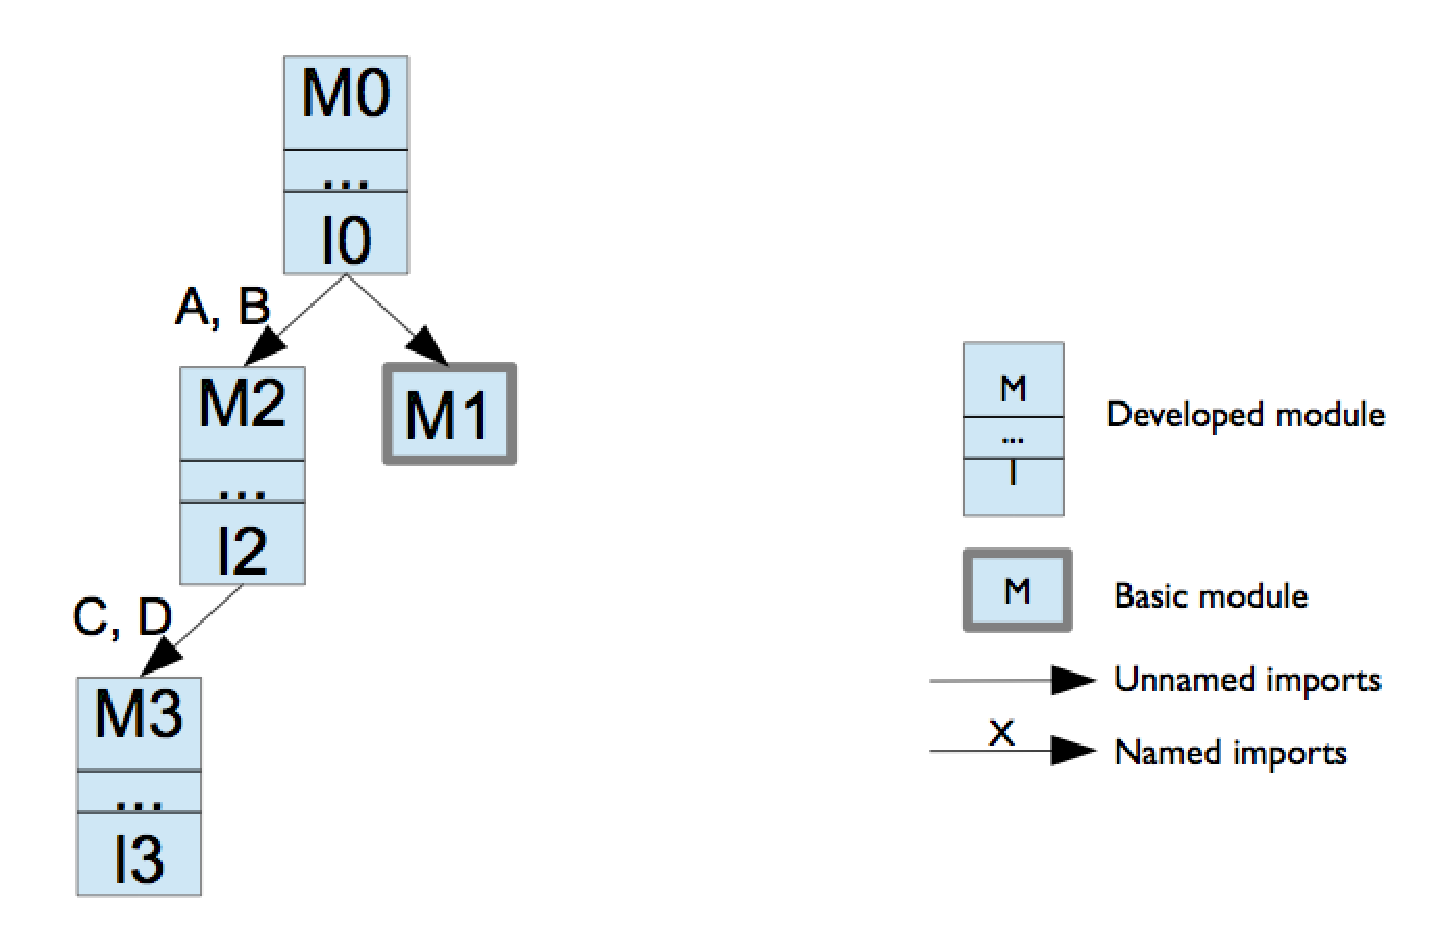
\includegraphics[width=.8\textwidth]{B-project.pdf}
\caption{Structure of the imports relation in a B project}
\label{fig:structure}
\end{center}
\end{figure}
Figure~\ref{fig:structure} illustrates this with the structure of a B project
where an implementation \B{I0} of a specification \B{M0} imports one unnamed
instance of a basic machine \B{M1} and two instances named \B{A} and \B{B} of a
developed machine \B{M2}. Its implementation \B{I2} in turn imports two
instances \B{C} and \B{D} of a developed machine \B{M3}, implemented as \B{I3}
(which has no imports itself).  

\section{Description of the input of the code generator}
\label{sec:b-ast}

We detail here the constructs that are considered in the compilation to the
LLVM. This description introduces the notations used in the definition of the
translation. The elements of the B language are denoted using a \B{sans serif}
font.

Figure~\ref{tab:node-attr} summarizes the structure
of the abstract syntax that is relevant in the definition of the proposed
translation and introduces identifiers used in the definition of the
translation. For instance, and for the purpose of the translation, the relevant
components of a B implementation are: \B{id}, the name identifying the
implementation within the project; \B{see}, a set of references to other modules
containing definitions used in the implementation; \B{const}, a set of constant
names, their type and their values; \B{impo}, a sequence of optionally
prefixed B machines corresponding to external modules instantiated in the
implementation; \B{var}, a set of variable names, their type and possibly
additional functional restrictions forming the rest of the state; \B{init}, a
sequence of instructions executed upon initialization of the implementation;
\B{op}, a set of operations, each being an algorithmic description of the
different functionalities provided by the implementation.

We distinguish the base module machines from developed module machines by
testing the \B{impl} attribute of the \B{Machine} element: if it is $\bot$, then
the machine is basic, otherwise it is the root of the corresponding
implementation.

The initialization and the operations are defined as (sequences of)
instructions. Operations also have a name, inputs and outputs. Possible
instructions are the classic imperative constructs: variable assignment, if and
case conditional, while loop, block with or without local variables, and
operation calls. The if constructs may have several branches, each with a
condition as well as an optional else branch. Called operations may be either
local operations or operations of instances of external modules, in this case
they have an optional prefix identifying the module.

Note that the translation presented in this paper only considers types \B{INT}
(integer) and \B{BOOL} (Boolean). Accordingly, the expression language consists
in arithmetic operations \B{-} (unary and binary), \B{+}, \B{*}, \B{/}, \B{mod},
% \B{**} (exponentiation),
\B{succ} and \B{pred} and Boolean operations
\B{$\land$}, \B{$\lor$}, \B{$\neg$} as well as relations \B{=}, \B{$\neq$},
\B{$>$}, \B{$<$}, \B{$\leq$} and \B{$\neq$}. Atomic expressions are identifiers,
Boolean constants \B{FALSE} and \B{TRUE}, integer literals, and integer
constants \B{MAXINT} and \B{MININT}. The development through the application of
the B method ensures the absence of overflows and underflows.

\begin{figure}[t]
  \begin{center}
    {\footnotesize
      \frame{
    \begin{tabular}[t]{ccccc}
      \begin{tabular}[t]{rcl}
        \hline
        \multicolumn{3}{|c|}{Machine: \B{Machine}} \\
        \hline
        \B{id} & : & \B{Name} \\
        \B{const} & : & seq \B{Cons} \\
        \B{var} & : & seq \B{Vari} \\
        \B{init} & : & seq \B{Inst} \\
        \B{op} & : & seq \B{Oper} \\
        \B{impl} & : & opt \B{Impl} \\
        \hline
        \multicolumn{3}{|c|}{Implementation: \B{Impl}} \\
        \hline
        \B{id} & : & \B{Name} \\
        \B{impo} & : & seq \B{Import} \\
        \B{const} & : & seq \B{Cons} \\
        \B{var} & : & seq \B{Vari} \\
        \B{init} & : & seq \B{Inst} \\
        \B{op} & : & seq \B{Oper} \\
        \hline
        \multicolumn{3}{|c|}{Imports: \B{Import}} \\
        \hline
        \B{mach} & : & \B{Machine} \\
        \B{pre} & : & opt \B{Name}
        \\
        \hline
        \multicolumn{3}{|c|}{Constant: \B{Cons}} \\
        \hline
        \B{id} & : & \B{Name} \\
        \B{type} & : & \B{Type} \\
        \B{val} & : & \B{Value} \\
        \hline
        \multicolumn{3}{|c|}{Variable: \B{Vari}} \\
        \hline
        \B{id} & : & \B{Name} \\
        \B{type} & : & \B{Type} \\
        \B{scope} & : & \B{Impl} \alt \B{Oper}
        \\
      \end{tabular}
      & &
      \begin{tabular}[t]{rcl}
        \hline
        \multicolumn{3}{|c|}{Operation: \B{Oper}} \\
        \hline
        \B{id} & : & \B{Name} \\
        \B{inp} & : & seq \B{Vari} \\
        \B{out} & : & seq \B{Vari} \\
        \B{body} & : & \B{Inst}
        \\
        \hline
        \multicolumn{3}{|c|}{Instruction: \B{Inst}} \\
        \hline
        \multicolumn{3}{c}{\B{Blk} \alt \B{VarD} \alt \B{If} \alt \B{BEq} \alt } \\
        \multicolumn{3}{c}{\B{Call} \alt \B{While} \alt \B{Case} \alt \B{Skip}} \\
        \hline
        \multicolumn{3}{|c|}{Block: \B{Blk}} \\
        \hline
        \B{body} & : & seq \B{Inst} \\
        \hline
        \multicolumn{3}{|c|}{Variable declaration: \B{VarD}} \\
        \hline
        \B{vars} & : & seq \B{Name} \\
        \B{body} & : & seq \B{Inst} \\
        \hline
        \multicolumn{3}{|c|}{If: \B{If}} \\
        \hline
        \B{branches} & : & seq \B{IfBr} \\
        \hline
        \multicolumn{3}{|c|}{Becomes equal: \B{Beq}} \\
        \hline
        \B{lhs} & : & \B{Vari} \\
        \B{rhs} & : & \B{Expr} \\
        \hline
        \multicolumn{3}{|c|}{Operation call: \B{Call}} \\
        \hline
        \B{op} & : & \B{Oper} \\
        \B{inp} & : & seq \B{Expr} \\
        \B{out} & : & seq \B{Name} \\
        \B{inst} & : & opt \B{Impo}
        \\
        \hline
        \multicolumn{3}{|c|}{Case conditional: \B{Case}} \\
        \hline
        \B{expr} & : & \B{Expr} \\
        \B{branches} & : & seq \B{CaseBr}
      \end{tabular}
      & &
      \begin{tabular}[t]{rcl}
        \hline
        \multicolumn{3}{|c|}{Case branch: \B{CaseBr}} \\
        \hline
        \B{val} & : & seq \B{Value} \\
        \B{body} & : & \B{Inst}
        \\
        \hline
        \multicolumn{3}{|c|}{While loop: \B{While}} \\
        \hline
        \B{cond} & : & \B{Pred} \\
        \B{body} & : & \B{Inst}
        \\
        \hline
        \multicolumn{3}{|c|}{If branch: \B{IfBr}} \\
        \hline
        \B{cond} & : & opt \B{Pred} \\
        \B{body} & : & \B{Inst} \\
        \hline
        \multicolumn{3}{|c|}{Expression: \B{Expr}} \\
        \hline
        \multicolumn{3}{c} {\B{Lit} \alt \B{Term} \alt \B{Pred} \alt \B{Vari}} \\
        \hline
        \multicolumn{3}{|c|}{Term expression: \B{Term}} \\
        \hline
        \B{op} & : & \B{ArithOp} \\
        \B{args} & : & seq \B{Exp} \\
        \hline
        \multicolumn{3}{|c|}{Predicate: \B{Pred}} \\
        \hline
        \multicolumn{3}{c}{\B{Form} \alt \B{Comp}} \\
        \hline
        \multicolumn{3}{|c|}{Boolean formula: \B{Form}} \\
        \hline
        \B{op} & : & \B{BoolOp} \\
        \B{args} & : & seq \B{Pred} \\
        \hline
        \multicolumn{3}{|c|}{Comparison: \B{Comp}} \\
        \hline
        \B{op} & : & \B{RelOp} \\
        \B{arg1}, \B{arg2} & : & \B{Exp} \\
        \hline
        \multicolumn{3}{|c|}{Data type: \B{Type}} \\
        \hline
        \multicolumn{3}{c}{\B{INT} \alt \B{BOOL}}
      \end{tabular}
    \end{tabular}
  }
  }
    \caption{Abstract syntax structure of a B implementation.  For each abstract
      syntax element, we give the name of the class (e.g. \B{CaseBr} for a
      branch in a case instruction, and the different attributes of the class),
      or a list of the possible sub-classes (e.g. \B{Inst} for the different
      kinds of instructions).
      Sequence and optional attributes are denoted ``seq'' and ``opt'',
      respectively}
    \label{tab:node-attr}
  \end{center}
\end{figure}

\section{Target LLVM Subset}
\label{sec:llvm}

LLVM aims to be a general, language agnostic, intermediate representation for
compilers. The compiler front-end translates the source programming language to
LLVM source code, upon which optimization and other static analysis tasks may be
performed, and the compiler back-end translates to the target platform assembly
language. One key feature of LLVM is that it is a single-static assignment (SSA)
language: a variable may only be assigned once. So for each assignment to a
variable found in the source language, the front-end shall generate a new
temporary variable in the LLVM program. For illustration,
figure~\ref{fig:ex-llvm} presents a LLVM program (for clarity, the corresponding
C code appears on the left) with two temporary variables \llvm{\%0} and
\llvm{\%1}.
\begin{figure}
\vspace*{-3em}
  \begin{minipage}[t]{.3\textwidth}
    \begin{tabbing}
      foo \= \kill  \\
      void inc(int * pi) \{\\
      \> *pi += 1; \\
      \}\end{tabbing}
  \end{minipage}
  \hfill
  \begin{minipage}[t]{.6\textwidth}
    \begin{tabbing}
      foo \= \kill  \\
      \llvm{define void @inc(i32* \%pi) \{} \\
      \llvm{entry:}                      \\
      \> \llvm{\%0 = load i32* \%pi}     \\
      \> \llvm{\%1 = add i32 \%0, 1}     \\
      \> \llvm{store i32 \%1, i32* \%pi} \\
      \> \llvm{ret void} \\
      \llvm{\}}
    \end{tabbing}
  \end{minipage}
  \caption{Simple example of a C function and its corresponding LLVM function.
    The first line contains the signature: return type \llvm{void}, the name
    \llvm{@inc} and one parameter named \llvm{\%pi} and typed \llvm{i32*}.  Next
    is the body with a single block, labeled \llvm{entry}, and temporary
    variables \llvm{\%0} and \llvm{\%1}, created in the conversion to SSA. The
    block has four instructions: \llvm{load}, \llvm{add}, \llvm{store} and
    \llvm{ret}. For instance, \llvm{\%1 = add i32 \%0, 1} is an addition
    (\llvm{add}), has result type \llvm{i32} and assigns to
    \llvm{\%1} the sum of variable \llvm{\%0} and integer
    literal \llvm{1}.}
  \label{fig:ex-llvm}
\end{figure}

The introduction to the LLVM that follows is focused in the features
that are relevant for the representation of B
implementations. Figure~\ref{fig:llvm-grammar} presents a grammar of this subset
of the LLVM.

\begin{figure}
  \begin{center}
    \begin{tabular}{rcl}
      \nt{module} & ::= & \ListOf{\nt{item}} \\
      \nt{item} & ::= & \nt{const\_decl} \alt \nt{function\_decl} \alt \nt{type\_def}
      \alt \nt{const\_def} \alt \nt{var\_def} \alt \nt{function\_def} \\
      \nt{const\_decl} & ::= & \nt{name} \llvm{=} \llvm{external} \llvm{constant} \nt{type} \\
      \nt{type\_def} & ::= & \nt{name} \llvm{=} \llvm{type} \nt{type} \\
      \nt{type} & ::= & \llvm{void} \alt \nt{itype} \alt \llvm{\{} \ListOf{\nt{type}} \llvm{\}} \alt \nt{type}\llvm{*} \\
      \nt{const\_def} & ::= & \nt{name} \llvm{=} \llvm{constant} \nt{type} \nt{iliteral} \\
      \nt{var\_def} & ::= & \nt{name} \llvm{=} \llvm{common} \llvm{global} \nt{type} \llvm{zeroinitializer} \\
      \nt{function\_decl} & ::= & \llvm{declare} \nt{type} \nt{name} \llvm{(} \ListOf{\nt{type}} \llvm{)}\\
      \nt{function\_def} & ::= & \llvm{define} \nt{type} \nt{name} \llvm{(} \ListOf{\nt{param}} \llvm{)} \llvm{\{} \ListOf{\nt{block}} \llvm{\}} \\
      \nt{param} & ::= & \nt{type} \nt{name} \\
      \nt{block} & ::= & \nt{lbl} \llvm{:} \ListOf{\nt{inst}} \\
      \nt{inst} & ::=  & \nt{name} \llvm{=} \llvm{alloca} \nt{type} \\
      & \alt & \nt{name} \llvm{=} \lalt \llvm{add} \alt \llvm{sub} \alt \llvm{mul} \alt \llvm{sdiv} \alt \llvm{srem} \ralt \nt{itype} \nt{exp} \llvm{,} \nt{exp} \\
      & \alt & \nt{name} \llvm{=} \llvm{icmp} \lalt \llvm{eq} \alt \llvm{ne} \alt \llvm{sgt} \alt \llvm{sge} \alt \llvm{slt} \alt \llvm{sle} \ralt \llvm{i1} \nt{exp} \llvm{,} \nt{exp}\\
      & \alt & \nt{name} \llvm{=} \llvm{call} \nt{type} \llvm{(} \ListOf{\nt{arg}} \llvm{)} \\
      & \alt & \nt{name} \llvm{=} \llvm{getelementptr} \nt{type} \llvm{*} \nt{exp}\llvm{,} \nt{index}\llvm{,} \nt{index} \\
      & \alt & \nt{name} \llvm{=} \llvm{load} \nt{type} \nt{exp} \\
      & \alt & \llvm{store} \nt{type} \nt{exp}, \nt{type} \llvm{*} \nt{exp} \\
      & \alt & \llvm{br} \llvm{i1} \nt{exp} \llvm{,} \llvm{label} \nt{lbl} \llvm{,} \llvm{label} \nt{lbl} \\
      & \alt & \llvm{br} \llvm{label} \nt{lbl} \\
%       & \alt & \llvm{switch} \nt{type} \nt{exp} \llvm{,} \llvm{branch} \nt{lbl} \llvm{[} \ListOf{\nt{branch}} \llvm{]} \\
      & \alt & \llvm{ret} \lalt \nt{type} \nt{exp} \alt \llvm{void} \ralt \\
      \nt{exp} & ::= & \nt{name} \alt \nt{iliteral} \alt \llvm{getelementptr} \llvm{(} \nt{type} \nt{exp} \llvm{,} \nt{index} \llvm{,} \nt{index} \llvm{)} \\
      \nt{index} & ::= & \nt{itype} \nt{iliteral} \\
      \nt{branch} & ::= & \nt{iliteral} \nt{iliteral} \nt{lbl} \\
      \nt{arg} & ::= & \nt{type} \nt{exp}
    \end{tabular}
  \end{center}
  \caption{Grammar of the target LLVM subset: \nt{itype}, \nt{iliteral}, \nt{lbl}
    and \nt{name} correspond respectively to integer types, integer literals,
    labels and names. Choices are separated by \alt and optionally delimited by
    \lalt and \ralt.  The \ListOf{} superscript denotes a comma-separated list of
    elements of the annotated entity.}
  \label{fig:llvm-grammar}
\end{figure}

LLVM programs are organized into modules\footnote{The term ``module'' has
  different meanings when considering the B method and LLVM.  We will use
  ``module'' for the former and ``LLVM module'' for the latter.}, one per
translation unit. A module may contain declarations of external entities
(functions, constants) and definitions of internal items (functions, variables,
constants). All data is explicitly typed. The name and type of external entities
must be declared.  All names, e.g. non-reserved identifiers, shall start with
\llvm{@}, when they are global, or\llvm{\%}, when they are local. For instance,
\llvm{@max = external constant i32} declares \llvm{@max} as a 32-bit integer
constant and \llvm{declare void @inc(i32*)} declares \llvm{@inc} as a function
having as parameter a pointer to an integer and \llvm{void} as a return type.

The type system contains the empty type \llvm{void}, an infinite, countable
number of integer types, one for each possible bit width (e.g. \llvm{i8} is the
type for 8-bit integers), and type constructors pointer (monadic \llvm{$\cdot$
  *}) and structure (polyadic \llvm{\{$\cdots$\}}). For instance \llvm{\{ i8*,
  i8, i8 \}} is the type for structures with three fields, the first having as
type pointer to \llvm{i8}. Grammar rule \nt{type\_def} states how types are
named, e.g.: \llvm{\%T1 = type \{i32, i32\}} and \llvm{\%T2 = type \{\%T1 *,
  \%T1 *\}}. Note that there is no \llvm{void *} type in the LLVM, instead
pointer values are of integer types.

Local entities are constants, variables or functions. An example of constant
definition is \llvm{@secret = constant i32 42}, it is composed of a name, type
and value. The elements of a variable definition are the name, type and code
generation attributes, e.g \llvm{@count = common global i32 zeroinitializer}.
Attributes \llvm{common}, \llvm{global} and \llvm{zeroinitializer} provide
information for target code generation: linkage type (the variable is merged
with other of the same name), the scope (global) and initialization of the
variable (zeroed is mandatory for common linkage). LLVM defines other attributes
for these aspects, but they are not needed in this work and their presentation
is omitted. For each such definition, a memory block is statically allocated to
stores the variable value. Function definitions are composed of the signature
and body. The signature contains the return type, name, parameters, and
attributes for target code generation. The body is a sequence of blocks of
instructions in single-static assignment (SSA) form, i.e., each
variable may be assigned exactly once.

The grammar rule \nt{inst} describes the different kind of instructions. All
instructions producing a value assign it to a fresh variable.  Instruction
\llvm{alloca} allocates a memory block the size of the given type on the stack
segment. This memory is automatically freed when the current frame is popped
from the stack. The LLVM does not include instructions for allocating from the
heap. Arithmetic operations are binary, and include signed quotient and
reminder. Arithmetic comparisons compare two values according to the first
operand and return a 1-bit integer value.  Instruction \llvm{call} invokes the
given function with the given arguments and assigns the result to a fresh
variable, which is of the given type.  In general, \llvm{getelementptr} gets the
address of an element in an aggregate object through indexing. In the target
LLVM subset, aggregate objects are structures, the first index has type
\llvm{i32} and value \llvm{0} to select the first structure at the given
location \nt{exp}, and the second index selects a field in that structure.
Instruction \llvm{load} assigns to a fresh variable \nt{name} the contents of a
memory address of type \nt{type} specified by \nt{exp} (e.g. in
fig.~\ref{fig:ex-llvm}).  Instruction \llvm{store} writes a value to memory
address (again, see fig.~\ref{fig:ex-llvm}).  Instruction \llvm{br} has two
forms.  In the first form, it directs conditionally the control flow to one of
two blocks.  If the given expression evaluates to \llvm{1}, control goes to the
first block, otherwise to the second. In the second form, the control jumps
unconditionally to the given block.
% Instruction \llvm{switch} directs the
% control flow to one of several blocks. The given expression is evaluated and
% control goes to the first branch with the matching value, or to the default
% branch (appearing first in the instruction).
Finally, instruction \llvm{ret}
ends the current function call, optionally returning a value.

The expression language is limited to names (local and global), integer literals
and selection of an element in a structure.

To conclude, we make no assumption on the existence of a library to obtain
resources managed by the operating system, such as dynamic memory allocation. In
the absence of such resource, all data must be allocated either statically, or
on the current stack frame, by using the \llvm{alloca} instruction.

\section{Translation: a global picture}
\label{sec:overview}

In addition to producing LLVM code that is faithful to the design developed in
B, our code generator is designed to satisfy the following two requirements:
\begin{description}
\item[static memory allocation] Many safety critical systems preclude use of
  this programming facility. All memory shall be allocated statically, save for
  the function call frame stack. As a side effect, no dynamic memory allocation
  library is required.
\item[separate compilation] An internal change in a module should only require
  generating new LLVM code for that module, and not for the modules that depend
  on it. This condition is important for large projects, where the development
  may be distributed to different persons.  If the change is in the interface
  though, the code generated from the dependent modules shall be updated.
\end{description}

We will use the example of the B project structure from
figure~\ref{fig:structure} to justify some decision taken in the design of the
code generator.  The example project consists of four modules. The corresponding
executable file shall include one instance of module \B{M0}, one instance of
\B{M1}, two instances of \B{M2} and four instances of \B{M3}. 

The module \B{M1} is basic, and we expect that the corresponding instance is
produced by another tool chain. Nevertheless, the LLVM code for \B{M0} may use
all the symbols defined in the interface of \B{M1} and we shall produce
corresponding LLVM declarations in the LLVM file for \B{M0}. Note that,
similarly, \B{M0} accesses the interface of \B{M2}, and \B{M2} accesses that of
\B{M3}.

\begin{quote}
  Given a module \B{M}, we need a procedure that generates the LLVM declarations
  for all the elements in the interface of \B{M}.
  The code produced by this procedure is called the \emph{interface section} of
  (the translation of) \B{M}.
\end{quote}

Now, consider that the modules have some data space. The LLVM code generator
needs to allocate memory to store the representation of the corresponding
data. Dynamic memory allocation being out of the picture, the sole solution is
static memory allocation, that is using global variables. Also, when the code
generator processes a B module, the number of instances there will be at run
time is not known, and we would not want to have to regenerate code each time
the module is used in a project to suit the number of instances. Indeed, the
best moment to instantiate the representation of the modules data space is when
the code for a whole project is generated.  

\begin{quote}
When generating code
for a given module, we need to consider the following two cases:
\begin{enumerate}
\item Code generation aims at producing a LLVM module,
  that will later be instantiated when generating the code for a project. We
  call this the \emph{COMP} mode for code generation.
\item Code generation is applied to build a full system from a project. Given
  the root module of the project, the code generator must identify all the
  transitively imported module instances. We call this the \emph{PROJ} mode for
  code generation.
\end{enumerate}
\end{quote}

The code generated for a module needs to address separately the representation
of the variables and the imported module instances. To do so, all the variables
and imported module instances are aggregated within a structure-like data
element. So, to encode the data space of a module, the code generator produces a
the definition of a LLVM structure type, named \llvm{\%M\$state\$}. This LLVM
definition is called the \emph{typedef section} of (the translation of) \B{M}.

However, to satisfy our second initial requirement (separate compilation), the
representation of the imported module instances cannot be part of the structure
itself.  Instead, the instances of the imported modules are represented as
references to the corresponding encoding structures (i.e., as pointers) are
used. We denote \llvm{\%M\$ref\$} the type pointer to \llvm{\%M\$state\$}.  

To encode behavior of a module, each operation \B{op} is translated into the
definition of a function named \llvm{@M\$op}. The parameter list of the
functions thus produced contains one item for each input and output of the
corresponding operation. There is also one parameter of type \llvm{\%M\$ref\$},
to pass the address of the instance encoding structure associated with that
operation. Also the translation produces a function \llvm{@M\$init\$}
responsible for executing the initialization of \B{M}. The parameters of this
function are the addresses of the instances found in the import tree of the
module (including the module itself). These parameters are necessary to call the
corresponding initialization functions and to bind the references to the
imported modules to elements of the structure of the initialized module. These
LLVM function definitions and the definition of the type \llvm{@M\$ref\$} form
the so-called the \emph{implementation section} of (the translation of) \B{M}.

\begin{figure}[t]
\begin{center}
\newcommand{\myind}{\hspace*{2em}}
\framebox{
\begin{minipage}{.9\textwidth}
\noindent\textbf{typedef section:}
Defines an LLVM data type \llvm{\%M\$state\$} corresponding to
the data space of the module: \\
\myind \llvm{\%M\$state\$ = type \{ \ListOf{\nt{type}} \}} \\
In case the data space of a module is empty, this section is empty and the
type is not defined. \\
\\
\noindent\textbf{interface section:} 
Defines an LLVM type \B{M\_ref}, pointer to \B{M\_data} (if
defined):\\
\myind \llvm{\%M\$ref\$ = type \%M\$state\$*} \\
The interface also contains declarations of one LLVM functions for each
operation of the module. \\
\myind \llvm{declare void @M\$op(\%M\$ref\$, \ListOf{\nt{type}})} \\
If the data space of the module is not empty, a function definition
corresponding to the initialisation is also emitted: \\
\myind \llvm{declare void @M\$init\$(\%M\$ref\$, \ListOf{\nt{type}})} \\
\\
\noindent\textbf{implementation section:}
Defines the functions declared in the interface (only for developed modules): \\
\myind \llvm{define void @M\$op(\%M\$state\$* \%self\$, \ListOf{\nt{param}}) \{} \\
\myind \myind \llvm{\ListOf{\nt{block}}} \\
\myind \myind \llvm{exit: ret void} \\
\myind \llvm{\}}
\end{minipage}
}
\end{center}
\caption{Summary of the different sections and the pattern of LLVM code
  composing them.}
\label{fig:summary}
\end{figure}

Figure~\ref{fig:summary} summarizes the three sections defined in our approach
for the code generation. These sections are combined differently in
\emph{PROJ\/} and \emph{COMP\/} mode. The \emph{COMP\/} translation assembles
them as follows:
\begin{center}
  \begin{tabbing}
    foo \= foo \= \kill
    \textit{for each imported module} \B{Q} \textit{generate} \\
    \> \llvm{\%Q\$state\$ = type opaque} \quad \textit{(declares type for} \B{Q} \textit{state space)} \\
    \> \textit{include the interface section of }\B{Q} \\
    \textit{include the typedef section of} \B{M} \\
    \textit{include the implementation section of} \B{M}
  \end{tabbing}
\end{center}
For a module \B{M}, the \emph{PROJ\/} translation is organized as follows:
\begin{center}
  \begin{tabbing}
    foo \= foo \= \kill
    \textit{for each transitively imported component} \B{Q} \\
    \> \textit{include the typedef section of \B{Q}} \\
    \textit{for each instance} \B{Q} \textit{imported transitively through} \B{path} \\
    \> \textit{declare a variable of type} \llvm{\%Q\$state\$}: \\
    \> \llvm{@Q$\lbrack$path$\rbrack$ = common global \%M\$state\$ zeroinitializer} \\

    \textit{for each imported component} \B{Q} \\
    \> \textit{include the interface section of} \B{Q} \\
    \textit{define a function} \llvm{\%\$init\$} \textit{with a call to the } \\
    \> \textit{initialization function of} \B{M} \textit{with the proper bindings} \\
    \> \llvm{define void @\$init\$(void) \{} \\
    \> \> \llvm{call void @M\$init\$(@M, \{ \ListOf{instances} \}) \{} \\
    \> \> \llvm{exit: ret void} \\
    \> \llvm{\}} \\
    \>
  \end{tabbing}
\end{center}

The following sections are devoted to the detailed presentation of the
translation of the different elements of a B implementation, as follows:
\begin{description}
\item[Notation] and some auxiliary definitions are presented in sec.~\ref{sec:notation}.
\item[Modularity] constructs to combine B components are described in
  sec.~\ref{sec:module}.
\item[Data] translation is briefly described sec.~\ref{sec:data}, including
  the encoding of B data types.
\item[Expressions] and conditions are codified as LLVM instruction blocks, as
  described in section~\ref{sec:expr}.
\item[Control] flow, instructions are translated to LLVM instructions as
  discussed in sec.~\ref{sec:control}, which also presents the encoding
  of B operations and initialization.
\end{description}

\section{Notations}
\label{sec:notation}

Code generation is defined with a set of rules defined by
structural recursion. For each grammatical construct, a code generation function
is defined: $\trad{~}{\B{Oper}}$ for operations, $\trad{~}{\B{Inst}}$ for
instructions, $\trad{~}{\B{Expr}}$ for expressions and so forth. Each such
function usually produces a text corresponding to bits of LLVM source code. It
may have additional parameter and results. The symbol $\sep$ is used to clearly
separate composed results. Auxiliary functions are introduced for
conveniency. To abbreviate the presentation, we denote
$\trad{~}{\ListOf{\B{A}}}$ as the translation function for sequences of \B{A}
elements, defined as the concatenation of the application of $\trad{~}{\B{A}}$
to the elements of the sequence.

In those rules, $\PH{t}$ indicates a text place-holder where the value of $t$
shall be inserted and $\nl$ denotes a new line. For instance, we define
$\local(\B{n}) \isdef \llvm{"\%\PH{\B{n.id}}"}$ as a function that given an
element \B{n} of the abstract syntax tree returns the corresponding LLVM local
name, obtained by prepending character \% to its identifier; and $\Global(\B{n})
\isdef \llvm{"@\PH{\B{n.root.id}}\$\PH{\B{n.id}}"}$ yields the corresponding
LLVM global name, composed by special characters (to avoid name conflicts), the
name of the component where it is defined and its own name.  Also, we define
additional auxiliary functions responsible for producing such identifiers:
\begin{align*}
\state(\B{n}) & \isdef \llvm{"\%\PH{\B{n.id}}\$state\$"} & \text{ (the type for the state)} \\
\stateref(\B{n}) & \isdef \llvm{"\%\PH{\B{n.id}}\$ref\$"} & \text{ (the type pointer to state)} \\
\init(\B{n}) & \isdef \llvm{"@\PH{\B{n.id}}\$init\$"} & \text{ (the initialization function)} \\
\self(\B{n}) & \isdef \llvm{"@\PH{\B{n.id}}\$self\$"} & \text{ (the instance in a top-level module)}
\end{align*}
We assume an unlimited supply of labels and local variables: we use $\lbl$ to
return a fresh LLVM label and $\variable$ for a fresh local variable name. Also, let us define:
\begin{itemize}
\item $\developed(\B{n}) \isdef \B{n.impl} \neq \bot$ to test if a machine is
  developed.
\item $\stateless(\B{n}) \isdef \B{n.vars} =  \bot \land \forall i \in \B{n.impo}, \stateless(i)$ to test if a machine is stateless.
\item $\importedmodules(\B{n}) \isdef \{ \B{i.mach} \mid \B{i} \in \B{n.impo}
  \}$ to get the set of machines directly imported from implementation $\B{n}$.
\item $\importedinstances(\B{n}) \isdef \B{n.impo}$ to get the set of machines
  instances directly imported from implementation $\B{n}$.
\item $\trimportedmodules(\B{n}) \isdef \ldots$ to get the set of machines
transitively imported from implementation $\B{n}$.
\item $\trimportedinstances(\B{n}) \isdef \ldots$ to get the set of machines
instances transitively imported from implementation $\B{n}$.
\item $\idx(\B{n}) \isdef \mathit{index}(\B{n}, \B{n.root.impo} \conc
  \B{n.root.vari})$ to get, from a given concrete variable $\B{n}$, the position
  of the corresponding element in the structure representing the state of the
  implementation. Here where $\mathit{index}(e, s)$ is a function that returns
  the position of $e$ in sequence $s$ and $\conc$ is the concatenation operator
  for sequences.
\end{itemize}

\section{Translation: Modularity Aspects}
\label{sec:module}

\subsection{The typedef section}

This section corresponds to the LLVM type definition for the state space of a
given module. If the module is developed, then the state space is that of the
corresponding implementation, otherwise the module is basic. If the basic
machine is stateless, the state space is empty; otherwise, it is represented by
an aggregate type, the elements of which correspond to the variables of the
machine:
\begin{align*}
  \trad{\B{n}}{\B{Mach}}_{\text{typedef}} \isdef
  & \IF \developed(\B{n}) \THEN \trad{\B{n.impl}, \B{n}}{\B{Impl}}_{\text{typedef}} \\
  & \ELSE \IF \stateless(\B{n}) \THEN \llvm{""} \\
  & \ELSE \llvm{"\PH{\state(\B{n})} = type \{ \PH{\trad{\B{n.vars}}{\ListOf{\B{Vari}}}_{\text{typedef}}} \} "}
\end{align*}

For the case of a developed machine \B{m} with implementation \B{n}, if \B{n} is
stateless, no type definition is emitted; otherwise, it is an aggregate type
composed of one element for each import and variable:
\begin{align*}
  \trad{\B{n}, \B{m}}{\B{Impl}}_{\text{typedef}} \isdef
  & \IF \stateless(\B{n}) \THEN \llvm{""} \\
  & \ELSE \llvm{"\PH{\state(\B{m})} = type \{ \PH{\trad{\B{n.impo}}{\ListOf{\B{Impo}}}_{\text{typedef}}}, \PH{\trad{\B{n.var}}{\ListOf{\B{Vari}}}_{\text{typedef}}} \} "}
\end{align*}

In these aggregate types, the elements corresponding to an import \B{n} is
defined in the following rule. If the imported machine is stateless, there is no
element, otherwise it is the name of the type pointer to the state of the
machine:
\begin{align*}
  \trad{\B{n}}{\B{Impo}}_{\text{typedef}} \isdef
  & \llvm{""} \triangleleft \stateless(\B{n.mach}) \triangleright \stateref(\B{n.mach})
\end{align*}

The elements corresponding to concrete variables are the LLVM data types
corresponding to the B types of those variables (defined in
sec.~\ref{sec:data}):
\begin{align*}
  \trad{\B{n}}{\B{Impl}}_{\text{typedef}} \isdef
  & \trad{\B{n.type}}{\B{Type}}
\end{align*}

\subsection{The interface section}

The interface section of a module \B{n} defines a type $\stateref(\B{n})$,
pointer to $\state(\B{n})$, the type to represent the data space of \B{n}, and
declares functions for executing 1) executing the initialization of an instance
of \B{n} and 2) each operation in \B{n}:
\begin{align*}
  \trad{\B{n}}{\B{Mach}}_{\text{interface}} \isdef
  & \llvm{"\PH{\stateref(\B{n})} = type \PH{\state(\B{n})}*\nl} \\
  & \llvm{\PH{\trad{\B{n}}{\B{init}}_{\text{interface}}}}\\
  & \llvm{\PH{\trad{\B{n.op}}{\ListOf{\B{Oper}}}_{\text{interface}}}"}
\end{align*}

The function responsible for initializing an instance of \B{n} takes as
parameter a reference to such instance, as well as a reference for each
transitively imported stateful instance and is as follows:
\begin{align*}
  \trad{\B{n}}{\B{init}}_{\text{interface}} \isdef
  & \llvm{"declare void \PH{\init(\B{n})} ( \PH{\stateref(\B{n})},
    \PH{\trad{\trimportedinstances(\B{n})}{\ListOf{\B{inst}}}_{\text{decl}}} )\nl"} \\
  \trad{\B{n}}{\B{inst}}_{\text{decl}} \isdef
  & \bot \triangleleft \stateless(\B{n.mach}) \triangleright \stateref(\B{n.mach})
\end{align*}

The function responsible for executing an operation \B{n} has as parameter a
reference to the instance of the corresponding module, if it is stateful, and
one parameter for each input and output of the corresponding operation:
\begin{align*}
  \trad{\B{n}}{\B{oper}}_{\text{interface}} \isdef
  &
\LET t = \bot \triangleleft \stateless(\B{n.root}) \triangleright \stateref(\B{n.root}) \IN \\
& \llvm{"declare void \PH{\Global(\B{n})}
( \PH{t},
  \PH{\trad{\B{n.inp}}{\ListOf{\B{Inp}}}_{\text{decl}}},
  \PH{\trad{\B{n.out}}{\ListOf{\B{Out}}}_{\text{decl}}}) \nl"} \\
  \trad{\B{n}}{\B{inp}}_{\text{decl}} \isdef & \trad{\B{n.type}}{\B{Type}} \\
  \trad{\B{n}}{\B{out}}_{\text{decl}} \isdef & \llvm{"\PH{\trad{\B{n.type}}{\B{Type}}}*"}
\end{align*}
It is noteworthy that the outputs of B operations are encoded as pointer
parameters.
\subsection{The implementation section}

The implementation section is composed of the definitions for each function
in the corresponding interface:
\begin{align*}
  \trad{\B{n}}{\B{Mach}}_{\text{implementation}} \isdef
  & \LET \B{i} = \B{n.impl} = \bot \IN\\
  & \quad \IF \B{i} = \bot \THEN \llvm{""} \\
  & \quad \ELSE \\
  & \quad \quad \llvm{"\PH{\trad{\B{i}}{\B{init}}}} \\
  & \quad \quad \llvm{\PH{\trad{\B{i.op}}{\ListOf{\B{Oper}}}}"}
\end{align*}
Code generation for operations and the initialization is described in
sec.~\ref{sec:control}.

\section{Translation: Data}
\label{sec:data}

The translation presented in this paper is currently limited to integers and
booleans. In the case of integers, the translation is based on the supposition
that the B0 definition of \B{INT} is the range $-2^{31}.. 2^{31}-1$. We have
$\trad{BOOL}{\B{Type}} \isdef \llvm{i1}$ and $\trad{INT}{\B{Type}} \isdef
\llvm{i32}$.

B constants shall be translated to constants in the LLVM program. The
translation of scalar constants consists in substituting them with their value.
\DD{The translation of non-scalar constants will be defined in a next version of
  this document.}  The definition of the translation for expressions is
described next in section~\ref{sec:expr}.

\section{Translation: Expressions}
\label{sec:expr}

To evaluate a composed expression using the LLVM, one must first generate a
sequence of instructions to evaluate each argument, the resulting value being
stored in a temporary variable, and second generate an instance of the LLVM
instruction corresponding to the expression argument.  Translation of
expressions is defined as functions that take as input some class of expressions
and produce a triple of strings $p \sep v \sep t$, where $p$ is a possibly empty
sequence of instructions required in the evaluation (e.g.  for the
sub-expressions), $v$ is the LLVM expression representing the resulting value,
and $t$ represents the LLVM type of the expression. In the case of composed
predicates, though, the evaluation is different as boolean operations need to be
implemented with conditional and unconditional jumps.

To facilitate the defintiion of rules that apply to similar cases, we introduce
mapping $\opmap$, that associates B operators to corresponding LLVM keywords:
$$\opmap = \{
\begin{array}[t]{l}
  = \mapsto \llvm{"eq"},
  \ne \mapsto \llvm{"ne"},
  < \mapsto \llvm{"slt"},
  \le \mapsto \llvm{"sle"},
  > \mapsto \llvm{"sgt"},
  \ge \mapsto \llvm{"sge"}, \\
  + \mapsto \llvm{"add"} \}.
  \end{array}
$$

\paragraph{Atomic expressions} have a simple translation. In the case of
literals, one only needs to issue the corresponding LLVM literal:
$\trad{TRUE}{\B{Lit}} \isdef \llvm{""} \sep \llvm{"1"} \sep \llvm{"i1"}$,
$\trad{FALSE}{\B{Lit}} \isdef \llvm{""} \sep \llvm{"0"} \sep \llvm{"i1"}$ and
$\trad{l}{\B{Lit}} \isdef \llvm{""} \sep \llvm{"\PH{l}"} \sep \llvm{"i32"}$ when
$\B{l.type} = \B{INT}$.

For identifiers, three cases are possible: global constants, local variables,
and module state variables. For state variables, the translation issues
statements to assign the address of the corresponding element in the state
structure to pointer variable $p$ and then dereference $p$ to assign $v$:
\begin{align*}
\lefteqn{\trad{n}{\B{Name}} \isdef \LET t = \trad{n.type}{\B{Type}} \IN} \\
& \IF \B{n} \mbox{ is a constant } \THEN \trad{n.value}{\B{Expr}} \\
& \ELSIF \B{n} \mbox{ is a local variable } \THEN
\llvm{""} \sep \local(\B{n}) \sep t \\
& \ELSE (\B{n} \mbox{ is a state variable }) \LET p = \variable \AND v = \variable \IN \\
& \quad \llvm{"\PH{p} = getelementptr \PH{\state(\B{n.root})} \%self\$, i32 0, i32 \PH{\idx(\B{n})} \nl} \\
& \quad \llvm{\PH{v} = load \PH{t}* \PH{p}\nl"} \sep v \sep t
\end{align*}

\paragraph{Comparisons} are formed by the application of a relational operator
to two expressions.

The code responsible for evaluating a comparison \B{r} is defined by the
following rule. First both arguments are evaluated in $p_1$ and $p_2$, and then
an instance of the LLVM comparison instruction \llvm{icmp} is used to compare
the temporary variables $v_1$ and $v_2$, of type $t_1 = t_2$, storing the result
in the fresh variable $v$.
\begin{align*}
\lefteqn{\trad{r}{\B{Comp}} \isdef
  \LET
  p_1 \sep v_1 \sep t_1 = \trad{r.arg1}{\B{Expr}} \AND
  p_2 \sep v_2 \sep t_2 = \trad{r.arg2}{\B{Expr}}} \\
& \IN \LET v = \variable \IN \\
& \llvm{"\PH{p_1}\quad\PH{p_2}\quad\PH{v} = icmp \PH{\opmap(\B{r.op})} \PH{t_1} \PH{v_1} \PH{v_2} \nl"} \sep v
\end{align*}

\paragraph{Arithmetic operations} have a similar
structure and interpretation as comparisons. Here is the rule for binary
arithmetic operations:
\begin{align*}
\lefteqn{\trad{r}{\B{Term}} \isdef
  \LET
  p_1 \sep v_1 \sep t_1 = \trad{r.arg1}{\B{Expr}} \AND
  p_2 \sep v_2 \sep t_2 = \trad{r.arg2}{\B{Expr}}} \\
& \IN \LET v = \variable \IN \\
& \llvm{"\PH{p_1}\quad\PH{p_2}\quad\PH{v} = i32 \PH{\opmap(\B{r.op})} \PH{t_1} \PH{v_1} \PH{v_2} \nl"} \sep v \sep \llvm{i32}
\end{align*}
Non-binary applications of associative operators are handled as nested
applications of binary applications. Next is the translation of the unary
\B{succ} operator:
\begin{align*}
  \trad{n}{\B{succ}} \isdef & \textbf{ let } p \sep v \sep t = \trad{n.arg}{\B{expr}} \IN  \\
  & \quad \LET w = \variable \IN \\
  & \quad \quad \llvm{"\PH{p}} \\
  & \quad \quad \llvm{\PH{w} = add i32 1, \PH{v} \nl"} \sep w \sep \llvm{i32}
\end{align*}

\paragraph{Predicates}
The translation of conditions takes as input a condition node \B{n}, as well as
two labels $\ell_t$ and $\ell_f$ that correspond to program locations where the
execution shall jump when the condition is evaluted to true or false,
respectively.  The first rule defines the translation of an atomic relation:
\begin{align*}
  \lefteqn{\trad{n, $\ell_t$, $\ell_f$}{\B{Form}} \isdef
  \textbf{ let } p \sep v = \trad{n}{\B{Comp}} \IN} \\
  & \llvm{"\PH{p} \quad br i1 \PH{v}, label \%\PH{\ell_t}, label \%\PH{\ell_f} \nl"}
\end{align*}

\noindent The translation for negation is simply: $\trad{not f, $\ell_t$,
  $\ell_f$}{\B{not}} \isdef \trad{f, $\ell_f$, $\ell_t$}{\B{Form}}$.  The
following rule handles the case of conjunctions. Note that it produces code with
a ``short-cut'' when the evaluation of the first argument yields false:
\begin{align*}
\begin{split}
  \lefteqn{\trad{n, $\ell_t$, $\ell_f$}{\B{and}} \isdef \LET \ell = \lbl \IN} \\
  & \LET p_1 = \trad{n.arg1, $\ell$, $\ell_f$}{\B{Form}}
  \AND p_2 = \trad{n.arg2, $\ell_t$, $\ell_f$}{\B{Form}} \IN \\
  & \quad \llvm{"\PH{p_1} \PH{\ell} :  \nl \PH{p_2}"}
\end{split}
\end{align*}
The definition of the translation for disjunctions is similar and is omitted.

\section{Translation: Control Flow and Instructions
\label{sec:control}}

This section addresses how operations in B implementations are translated to
LLVM functions. It also discusses initialization, which might be seen as a
special kind of operation. For operations, the presentation of the translation
is divided into three steps: the signature, the local data, and the body
instructions.

The signature of the function is composed of the name of the function, the
result type, the name and type of the parameters. The signature may carry other
information such as linkage, visibility, calling convention, etc. The B parser
provides this information after the type checking phase has been completed.  On
the one hand LLVM functions may only have one result, on the other hand B0
operations may produce several results. The translation of output parameters
will be function parameters passed by reference, i.e. they are pointers. For
uniformity of treatment, the return type of the produced LLVM functions is
\llvm{void}. Translation of operation headers is defined in
sec.~\ref{sec:trad-header}. The memory to store local variables is allocated on
the stack, using the \llvm{alloca} instruction. We describe a function in
sec.~\ref{sec:trad-alloc} that, applied to a B operation, returns the name and
type of its local variables used in the operation. These names are translated to
conform to LLVM restrictions. The body of the operation has to be transformed to
a sequence of LLVM blocks of statements. For each kind of instruction one (or
more) translation function is defined. The details are provided in
section~\ref{sec:trad-instr}.  The results of the translation of each aspect are
combined as follows:
\begin{align*}
\begin{split}
  \lefteqn{\trad{\B{op}}{\B{oper}} \isdef} \\
  & \LET h = \trad{\B{op}}{sig} \AND   a = \trad{\B{op.body}}{alloc} \AND i = \trad{\B{op.body}, \llvm{exit}}{\ListOf{\B{Inst}}}_L \IN  \\
  & \llvm{"define void \PH{h} \{\nl} \\
  & \quad \llvm{entry:\nl} \\
  & \quad \quad \PH{a} \\
  & \quad \quad \PH{i} \\
  & \quad \llvm{exit: ret void\nl} \\
  & \llvm{\}\nl"}
\end{split}
\end{align*}

Initialization of a B implementation shares many characteristics with operations
but needs to deal with initialization of imported modules. It is discussed in
sec.~\ref{sec:trad-init}.

\subsection{Sub-routines signatures}
\label{sec:trad-header}

The following rule specifies the translation of operation headers. Its
parameters are the operation identifier, inputs, outputs, the name of the
machine it belongs to, and the results are the LLVM function definition
header: \\
\noindent$\trad{\B{o}}{sig} \isdef \llvm{"\PH{\Global(\B{o})}(\PH{\state(\B{o.root})}* \%self\$, \PH{\trad{\B{o.inp}}{\ListOf{inp}}}, \PH{\trad{\B{o.out}}{\ListOf{out}}})"}$

Next are the rules defining the translation of individual input and output
parameters. They have local scope and they are translated by prepending
\llvm{\%}:
\begin{align*}
  \trad{i}{inp} \isdef
  \llvm{"\PH{\trad{i.type}{\B{Type}}} \PH{\local(\B{i})}"} \quad \quad
  \trad{o}{out} \isdef
  \llvm{"\PH{\trad{o.type}{\B{Type}}}* \PH{\local(\B{o})}"}
\end{align*}

\subsection{Stack allocation}
\label{sec:trad-alloc}

B operations may have local variables, in which case the translator needs to
issue LLVM stack allocation instructions. Such instructions have two arguments:
the type of values to store, and a temporary variable that is assigned the
address (see figure~\ref{fig:llvm-grammar} for the concrete syntax). The
generation of stack allocation code visits the parse tree of the operation body
in a pre-order depth-first traversal, generating one statement for each local
variable declaration found. The detailed definition of this traversal is omitted
for space reasons. For each B0 variable \B{v} found, a LLVM name is thus
created.
\begin{align*}
  \trad{v}{alloc} \isdef
  \llvm{"\PH{\local(\B{v})} = alloca \PH{\trad{v.type}{\B{Type}}} \nl"}
\end{align*}

After the stack allocations, the LLVM source code contains the statements that
encodes the instructions in the body of the operation, as described in the
following section.

\subsection{Translation of instructions}
\label{sec:trad-instr}

One issue in the translation of instructions is the disruption of the flow graph
intro a linear sequence of instructions and branches. This requires the creation
of instruction labels. As a consequence, our definition of the translation of
instructions has two kinds of rules, those that take a label as parameter, and
those that do not. Such label parameter indicates where the control should go
after the corresponding execution is executed.

\begin{align*}
\trad{\B{i}, $\ell$}{\B{Inst}}_L \isdef
& \IF \B{i} \mbox{ is \B{If}} \THEN \trad{\B{i}, $\ell$}{\B{If}}_L \\
& \ELSIF \B{i} \mbox{ is \B{While}} \THEN \trad{\B{i}, $\ell$}{\B{While}}_L \\
& \ELSIF \B{i} \mbox{ is \B{Blk}} \THEN \trad{\B{i.body}, $\ell$}{\ListOf{\B{Inst}}}_L \\
& \ELSE \LET p = \trad{\B{i}}{\B{Inst}} \IN \\
& \quad \llvm{"\PH{p}} \\
& \quad \llvm{ br label \%\PH{\ell} \nl"}
\end{align*}

Function $\trad{\B{il}, $\ell$}{\ListOf{\B{Inst}}}_L$ takes as input a sequence
of B instructions \B{il} and a label $\ell$ and produces the source code of a
LLVM block with $\ell$ as exit point. It is defined as follows:

\begin{align*}
\trad{\B{il}, $\ell$}{\ListOf{\B{Inst}}}_L \isdef & \IF \B{il} \mbox{ is empty} \THEN \llvm{"br label \%\PH{\ell} \nl"} \\
& \ELSE \\
& \LET \B{i}, \B{il'} = \B{il}  \IN \\
& \quad \quad \LET p_1 =
\begin{array}[t]{l}
  \IF \B{i} \mbox{ is \B{If} or \B{While}} \THEN \\
  \quad \LET \ell' = \lbl \IN \llvm{"\PH{\trad{i, $\ell'$}{\B{Inst}}_L} \PH{\ell'}: \PH{p}"} \\
  \ELSE \llvm{"\PH{\trad{i}{\B{Inst}}} \PH{p}"} \IN
\end{array} \\
& \quad \quad \IN \\
& \quad \quad \quad \llvm{"\PH{p_1}} \\
& \quad \quad \quad \llvm{\PH{\trad{il', $\ell$}{\ListOf{\B{Inst}}}_L}"}
\end{align*}

Eventually, $\trad{}{\B{Inst}}$ defines the translation for individual
instructions. Its definition is specialized for each class of instructions as
detailed in the rest of this section. Note that a new block is created after
each \B{If} and \B{While} instruction.

\paragraph{Becomes equal instructions} must evaluate the target and the source
of the assignment, and then copy the result of the latter in the former, using
the LLVM instruction \llvm{store}. The evaluation of the target is defined with
$\trad{}{lv}$, which yields the corresponding LLVM source code $l$ and the
variable $p$ containing the assigned location. The evaluation of the source
yields the corresponding code $r$, the variable $v$ holding the result, and its
type $t$.
\begin{align*}
\begin{split}
  \trad{a}{\B{Beq}} \isdef
  & \LET l \sep p \sep t'= \trad{i.lhs}{lv} \AND r \sep v \sep t = \trad{i.rhs}{\B{Expr}} \IN \\
  & \llvm{"\PH{l}} \\
  & \llvm{\PH{r}} \\
  & \llvm{store \PH{t} \PH{v}, \PH{t'} \PH{p} \nl"}
%   & l \conc r \conc
%   \llvm{"store "} \conc t \conc \texttt{" "} \conc v \conc \llvm{", "}
%   \conc t \conc \llvm{"* "} \conc p \conc \nl
\end{split}
\end{align*}
The assignment target may be either local to the operation or a state
variable. In the former case, it can be referenced by the corresponding LLVM
identifier. In the latter case, it is represented as an element of the state
structure $\Sigma$, and its address must be calculated and assigned to a new temporary
variable.
\begin{align*}
\lefteqn{\trad{n}{lv} \isdef} \\
& \LET t = \llvm{"\PH{\trad{\B{n.type}}{Type}} *"} \IN \\
& \quad \IF \mbox{\B{n} is a local variable} \THEN \llvm{""} \sep \local(\B{n}) \sep t \\
& \quad \ELSE \LET v = \variable \IN \\
& \quad \quad \llvm{"\PH{v} = getelementptr \PH{\state(\B{n.root})}* \%self\$,} \\
& \quad \quad \quad \llvm{i32 0, i32 \PH{\idx(\B{n})} \nl"} \sep v \sep t
\end{align*}

\paragraph{Call up} instructions apply B operations with some values and obtain
results. The LLVM code generator produces instructions to evaluate the operation
arguments, the address of the variables receiving the results as well as an
instance of the LLVM \llvm{call} instruction. In addition, the proposed
translation includes as argument the address of a structure storing the state of
the component corresponding to this operation. Note that this component may be
either the implementation being translated (in the case of a so-called local
operation), or an instance of an imported machine.
\begin{align*}
  \trad{c}{\B{Call}} \isdef
  & \LET p_i \sep il = \trad{c.inp}{\ListOf{Inp}} \AND p_o \sep ol =
  \trad{c.out}{\ListOf{Out}} \AND \\
  & \quad id = {\Global(\B{c})} \AND ty = \llvm{"\PH{\stateref(\B{c.root})}} \AND \\
  & \quad val \sep p = \IF \B{c.inst} = \text{None} \\
  & \quad \quad \THEN \llvm{"\%self\$"} \sep \llvm{""} \\
  & \quad \quad \ELSE \LET v_1, v_2 = \variable, \variable \IN \\
  & \quad \quad \quad v_2 \sep \\
  & \quad \quad \quad \llvm{"\PH{v_1} = getelementptr \PH{ \state({\B{c.inst.root}})} \%self\$, i32 0, i32 \PH{\idx(\B{c.inst})} \nl} \\
  & \quad \quad \quad \quad \llvm{\PH{v_2} = load \PH{ty}* \PH{v_1} \nl"} \\
  & \IN \\
  & \quad \llvm{"\PH{p_i}} \\
  & \quad \llvm{\PH{p_o}} \\
  & \quad \llvm{\PH{p}} \\
  & \quad \llvm{call void \PH{id}(\PH{ty} \PH{val}, \PH{il}, \PH{ol}) \nl"}
\end{align*}
The translation of input and output arguments produces two code snippets. The
first corresponds to the LLVM instruction sequence $p$ responsible for
evaluating the argument, and the second to the type $t$ and name $v$ of the
variable storing the resulting value:
\begin{align*}
  \trad{i}{Inp} \isdef
  & \LET p \sep v \sep t = \trad{i}{\B{Expr}} \IN p \sep \llvm{"\PH{t} \PH{v}"}\\
  \trad{o}{Out} \isdef
  & \LET p \sep v \sep t = \trad{o}{lv} \IN p \sep \llvm{"\PH{t} \PH{v}"}
\end{align*}

\paragraph{Identity} does nothing and no code is generated:
\begin{align*}
\begin{split}
  \trad{n}{\B{Skip}} \isdef & \llvm{""}
\end{split}
\end{align*}

\paragraph{Block instructions} are structuring constructs that have no
operational intent; their translation is that of their body: $\trad{i,
  $\ell$}{\B{Blk}} \isdef \trad{i.body, $\ell$}{\ListOf{\B{Inst}}}$.


\paragraph{If instructions} are sequences of possibly conditional blocks of
instructions, i.e. branches. After a branch is executed, control must go
to the next block $\ell$.
\begin{align*}
  \trad{i, $\ell$}{\B{If}}_L \isdef \trad{i.branches, $\ell$}{\ListOf{\B{IfBr}}}
\end{align*}
To translate conditional branches, one must first generate code to evaluate the
condition of the branch, followed by an LLVM conditional branching statement,
translate the body of the branch, and add an unconditional branch to the block
following the corresponding \B{If} statement.  The translation for branches has
as arguments a branch \B{b}, the remaining branches \B{bl}, the lexicon, and the
label $\ell$ of the block following the \B{If} statement they belong to. The
following definition applies for the case of conditional branches:
\begin{align*}
\begin{split}
  \trad{\B{b bl}, $\ell$}{\ListOf{\B{IfBr}}} \isdef & \LET \ell_1 = \lbl \AND \ell_2 = \lbl \IN \\
  & \llvm{"\PH{\trad{b.cond, $\ell_1$, $\ell_2$}{\B{Pred}}} } \\
  & \llvm{\PH{\ell_1} : \PH{\trad{b.body, $\ell$}{\ListOf{\B{Inst}}}_L}} \\
  & \llvm{\PH{\ell_2} : \PH{\trad{bl, $\ell$}{\ListOf{\B{IfBr}}}}"} \\
\end{split}
\end{align*}
The following rule handles the case of the last branch, which might have a condition or not:
\begin{align*}
\begin{split}
  \trad{\B{b}, $\ell$}{\ListOf{\B{IfBr}}} \isdef & \IF \B{b.cond} = \text{None} \THEN
  \trad{b.body, $\ell$}{\ListOf{Inst}}_L\\
  & \ELSE \LET \ell_1 = \lbl \IN \\
  & \llvm{"\PH{\trad{b.cond, $\ell_1$, $\ell$}{\B{Pred}}} } \\
  & \llvm{\PH{\ell_1} : \PH{\trad{b.body, $\ell$}{\ListOf{\B{Inst}}}_L}}
\end{split}
\end{align*}

\paragraph{Case instructions} are formed by an expression, and a list of case
branches, each of which has a list of values and an instruction block.
Optionally, there might be a default branch, and we consider that, in this case,
the list of values is empty.

The translation to the LLVM IR uses its switch statement. It is composed of a
variable, a default jump and a jump table. The jump table is a sequence of pairs
formed by a value, and an instruction label. In the following, \llvm{\%val} is
the variable, \llvm{\%otherwise} is the default label, and the jump table has
three entries. The first corresponds to the case where the value of \llvm{\%val}
is \llvm{0}, in which case the execution jumps to the label \llvm{onzero}.
\begin{verbatim}
switch i32 %val, label %otherwise [ i32 0, label %onzero
                                    i32 1, label %onone
                                    i32 2, label %ontwo ]
\end{verbatim}

The translation of the case statement first consists in producing the code $p$
to evaluate the expression tested in the statement. When that code completes
execution, the value is stored in variable $v$ of type $t$. Then the jump table
$j$ and the code $b$ of the different branches are generated. This generation
takes also as parameters labels $\ell$ and $\ell_o$.
\begin{align*}
  \trad{v, $\ell$}{\B{Case}} \isdef & \LET p \sep v \sep t = \trad{v.expr}{\B{Expr}} \IN \\
  & \LET \ell_o = \lbl \IN \\
  & \LET j, b = \trad{v.branches, $\ell_o$, $\ell$}{\ListOf{CaseBr}} \IN \\
  & \quad \llvm{"\PH{p}} \\
  & \quad \llvm{switch \PH{t} \PH{v}, label \%\PH{\ell_o} [ \PH{j} ] \PH{b}"}
\end{align*}

The following rule defines the composition of the translation of the different
branches of a case statement. Again, this translation has two parts: bits of the
jump table $j$, and instruction blocks $b$. If a case branch has several values,
then several entries need to be created in the jump table. This is the role
of the translation function $\trad{}{\B{ListOf{CaseVal}}}$.
\begin{align*}
  \trad{b bl, $\ell_o$, $\ell_e$}{\ListOf{\B{CaseBr}}} \isdef
  & \LET \ell = \lbl \IN \\
  & \LET j, b = \trad{bl, $\ell_o$, $\ell_e$}{\ListOf{\B{CaseBr}}} \IN \\
  & \quad \llvm{"\PH{\trad{b.values, $\ell$}{\ListOf{\B{CaseVal}}}} \PH{j}"}
  \sep \\
  & \quad
  \llvm{"\PH{\ell}: \nl \PH{\trad{b.body, $\ell_e$}{\ListOf{Inst}}_L} \PH{b}"}
\end{align*}
This rule handles the last branch of a case statement, and needs to test if
that branch is a default branch or not. If not, then one needs to be artificially
created (as this is mandatory in the LLVM-IR switch statement):
\begin{align*}
  \trad{b, $\ell_o$, $\ell_e$}{\ListOf{\B{CaseBr}}} \isdef
  & \IF \B{b.values} = \text{None} \THEN \\
  & \quad \llvm{""} \sep \llvm{"\PH{\ell_o}: \nl \PH{\trad{b.body, $\ell_e$}{\ListOf{Inst}}_L}"} \\
  & \ELSE \LET \ell_b = \lbl \IN \\
  & \quad \trad{b.values, $\ell_b$}{\ListOf{\B{CaseVal}}} \sep \\
  & \quad \llvm{"\PH{\ell_b}: \nl \PH{\trad{b.body, $\ell_e$}{\ListOf{Inst}}_L}} \\
  & \quad \quad \llvm{\PH{\ell_o}: \nl br label \% \PH{\ell_e}}
\end{align*}

The following rules specifies that the values of a case branch are translated in
order, their translations being concatenated to form the result. The parameter
$\ell$ is the label of the instruction block containing the translation of the
branch body:
\begin{align*}
  \trad{v, $\ell$}{\ListOf{\B{CaseVal}}} \isdef & \trad{v, $\ell$}{\B{CaseVal}} \\
  \trad{v vl, $\ell$}{\ListOf{\B{CaseVal}}} \isdef &
  \llvm{"\PH{\trad{v, $\ell$}{\B{CaseVal}}} \PH{\trad{vl, $\ell$}{\ListOf{\B{CaseVal}}}}"}
\end{align*}

This rule defines how a single value of a case branch is translated, namely
as an entry in the jump table of a switch statement:
\begin{align*}
  \trad{v, $\ell$}{\B{CaseVal}} \isdef & \LET p \sep v \sep t = \trad{v}{\B{Expr}} \IN \\
  & \quad \llvm{"\PH{t} \PH{v}, label \%\PH{\ell} \nl"}
\end{align*}

\paragraph{While instructions} are translated in two blocks of instructions:
block $\ell_1$ evaluates the loop condition and block $\ell_2$ executes the loop
body:
\begin{align*}
\begin{split}
\trad{w, $\ell$}{\B{While}} \isdef
  & \LET \ell_1 = \lbl \AND \ell_2 = \lbl \AND c \sep v = \trad{w.cond}{\B{Pred}} \IN \\
  & \llvm{"br label \%\PH{\ell_1} \nl} \\
  & \llvm{\PH{\ell_1} : \PH{c}} \\
  & \llvm{br i1 \PH{v}, label \%\PH{\ell_2}, label \%\PH{\ell} \nl} \\
  & \llvm{\PH{\ell_2} : \PH{\trad{i.body, $\ell_1$}{\ListOf{\B{Inst}}}_L}}
\end{split}
\end{align*}

\subsection{Initialization}
\label{sec:trad-init}

[[[ DEPRECATED ]]]

Initialization is done is two steps: first all imported modules are
initialized,  second the initialization clause is executed.
\begin{align*}
  \trad{i}{Init} \isdef
  & \llvm{"define void @\PH{\B{i.id}}\$init\$() \{ \nl"} \\
  & \quad\llvm{\PH{\trad{i, i.impl}{\ListOf{InitImp}}}} \\
  & \quad\llvm{\PH{\trad{i.init, "exit"}{\ListOf{\B{Inst}}}_L}} \\
  & \quad\llvm{exit: ret void \nl} \\
  & \llvm{\}"}
\end{align*}
The initialization of an imported module is performed by a call to the
corresponding initialization function:
\begin{align*}
  \lefteqn{\trad{\B{impl}, \B{impo}}{InitImp} \isdef} \\
  & \LET v = \variable \AND \B{m} = \B{impo.mach} \IN \\
  & \quad \llvm{"\PH{v} = getelementptr \PH{\state(\B{impl.root})}* \%self\$, i32 0, i32 \PH{\idx(\B{impo})}\nl}\\
  & \quad \llvm{call void @\PH{\B{m.id}}\$init\$(\PH{\state(\B{m.impl})}*
    \PH{\ell}) \nl"}
\end{align*}

\section{Validation}
\label{sec:validation}

To validate the rules defining the code generator, we follow a pragmatic
approach, based on testing and simulation of the generated LLVM artifacts, and
using the existing LLVM tool set. The rules described in the preceding sections
have been prototyped in the Python programming language. The input of the
translation is in a XML-based format, named BXML, that is generated by the
forthcoming version of Atelier-B. For each B component (machine or
implementation), Atelier-B generates a BXML file that may then be used as input
by our prototype. The output of the translation is LLVM code. Such output may
then be processed by the LLVM tools either to generate binary in some compatible
target platform or LLVM bitcode that may then be executed using the LLVM
interpreter. We used the latter approach to validate our translation.

The LLVM tools that are employed are:
\begin{description}
\item[llvm-as] The LLVM assembler generates LLVM bitcode, invoked, e.g., as
  follows:
\begin{verbatim}
llvm-as example-01.llvm -o example-01.bc
\end{verbatim}
\item[llvm-link] The LLVM bitcode linker, which may be invoked as follows:
\begin{verbatim}
llvm-link example-01.bc example-02.bc -o prog.bc
\end{verbatim}
\item[lli] The LLVM bitcode interpreter, which may be invoked as follows:
\begin{verbatim}
lli example-01.bc
\end{verbatim}
\end{description}

We describe below the different commands required to use the LLVM framework to
animate a B implementation \B{wd} that uses an instance of a B module
\B{counter}:
\begin{verbatim}
b2llvm counter counter.llvm
b2llvm wd counter.llvm
b2llvm --mode proj wd init-wd.llvm
llvm-as counter.llvm -o counter.bc
llvm-as wd.llvm -o wd.bc
llvm-as init-wd.llvm -o init-wd.bc
llvm-as scaffold-wd.llvm -o scaffold-wd.bc
llvm-link counter.bc wd.bc init-wd.bc scaffold-wd.bc -o anim-wd.bc
lli anim-wd.bc
\end{verbatim}


\section{Conclusion and future work}
\label{sec:conclusion}

This paper presents the formal specification of a translation from a large
subset of the B implementation language to LLVM, a modern compiler internal
language.  Even though this is still a work in progress, the definition is
self-contained and has a large enough scope to be applied to B implementations
where the data belongs to basic types. This specification is a blueprint for a
code synthesis tool for B that is currently being implemented. This tool will be
distributed as an extension to Atelier-B under an open-source license.

The next step is to extend the scope to the full B implementation language. This
entails that the translation must be defined for aggregate data types and
adapted to handle some syntactic sugar. We are also planning for producing a
LLVM output with debugging information. Such output would be indeed very helpful
to provide feedback to the user when applying testing to validate the produced
code.

To prove the verification of the correctness of the translation, we would have
to define the semantics of both LLVM and B in a unified framework. One possible
starting point is Vellvm~\cite{vellvm}, a framework to reason about the
correctness of LLVM programs and transformations. We would then have to extend
the framework to include B implementation language. Another possible approach
would be to translate verification conditions from the B development artifacts
as assertinons in the generated LLVM code. The compiled program would include
checks that such assertions hold while executing.

\bibliographystyle{plain}
\bibliography{b2llvm}

\newpage
\appendix

\section{Test summary}

For each test file, indicates the B0 constructs found in the implementation.
\begin{center}
\newcommand{\no}[0]{--}
\newcommand{\yes}[0]{$\circ$}
\begin{tabular}{|l|c|c|c|c|c|c|c|c|}
\hline
Example nº & 01 & 02 & 03 & 04 & 05 & 06 & 07 & 08 \\
\hline
\hline
\multicolumn{9}{|c|}{clauses} \\
\hline
import w.o prefix & \no & \no & \no & \no & \no & \no & \yes & \no \\
import w prefix & \no & \no & \no & \no & \no & \no & \no & \yes \\
variables & \yes & \yes & \yes & \yes & \yes & \yes & \no & \yes \\
constants & \no & \yes & \no & \no & \yes & \no & \yes & \yes \\
op. input & \yes & \no & \yes & \no & \no & \no & \no & \no \\
op. output & \yes & \no & \yes & \no & \no & \no & \yes & \yes \\
\hline
\multicolumn{9}{|c|}{instructions} \\
\hline
block & \yes & \no & \yes & \yes & \no & \yes & \no & \yes \\
local var & \no & \no & \yes & \yes & \no & \yes & \yes & \yes \\
identity & \no & \no & \yes & \no & \no & \no & \no & \no \\
becomes equal & \yes & \yes & \yes & \yes & \yes & \yes & \yes & \yes \\
operation call & \no & \no & \no & \no & \no & \no & \yes & \yes \\
condition & \yes & \no & \no & \no & \yes & \no & \yes & \yes \\
case & \no & \no & \no & \no & \no & \yes & \no & \no \\
assertion & \no & \no & \no & \no & \no & \no & \no & \no \\
sequence & \yes & \yes & \yes & \yes & \no & \yes & \yes & \yes \\
while & \no & \no & \no & \yes & \no & \no & \yes & \no \\
\hline
\multicolumn{9}{|c|}{types} \\
\hline
INT & \yes & \yes & \yes & \yes & \yes & \yes & \yes & \yes \\
BOOL & \yes & \yes & \no & \no & \yes & \no & \yes & \yes \\
\hline
\multicolumn{9}{|c|}{expressions} \\
\hline
int lit & \yes & \yes & \yes & \yes & \yes & \yes & \yes & \yes \\
bool lit & \yes & \yes & \no & \yes & \yes & \no & \yes & \yes \\
vars & \yes & \yes & \yes & \yes & \no & \yes & \no & \yes \\
loc. vars & \no & \no & \yes & \yes & \no & \yes & \yes & \yes \\
const & \no & \yes & \no & \no & \yes & \no & \yes & \yes\\
succ & \no & \yes & \no & \yes & \yes & \no & \no & \no \\
pred & \no & \yes & \no & \yes & \yes & \no & \no & \no \\
+ & \yes & \no & \no & \yes & \no & \yes & \yes & \no \\
- & \yes & \no & \no & \no & \no & \no & \yes & \no \\
* & \no & \no & \no & \no & \no & \yes & \no & \no \\
\hline
\multicolumn{9}{|c|}{formulas} \\
\hline
and & \no & \no & \no & \no & \yes & \no & \no & \no \\
or & \no & \no & \no & \no & \yes & \no & \no & \no \\
not & \no & \no & \no & \no & \yes & \no & \no & \no \\
$<$ & \yes & \yes & \no & \no & \no & \no & \yes & \yes \\
$>$ & \no & \no & \no & \no & \yes & \no & \yes & \no \\
\hline
\end{tabular}
\end{center}


\end{document}
